\documentclass[12pt]{article}
\usepackage{amsmath}
\usepackage{fancyhdr}
\usepackage{geometry}
\usepackage{parskip}
\usepackage{pdfpages}
\usepackage{graphicx}
\usepackage{mathtools}

\graphicspath{{./}}
\geometry{letterpaper, portrait, margin=1in}
\setlength{\parindent}{0pt}

\title{Math 252 Homework\\
\large Sections 6.1 \& 6.2}
\date{2016/04/24}
\author{Solomon Greenberg}

\fancyhf{}
\pagestyle{fancy}

\lhead{Math 252 Homework --- Section 6.1 \& 6.2}
\rhead{Solomon Greenberg}

\newcommand{\me}{\mathrm{e}}
\newcommand{\dx}{\mathrm{d}x}
\newcommand{\dtheta}{\mathrm{d}\theta}
\newcommand{\md}{\mathrm{d}}
\DeclarePairedDelimiter\abs{\lvert}{\rvert}%
\DeclarePairedDelimiter\norm{\lVert}{\rVert}%

% Swap the definition of \abs* and \norm*, so that \abs
% and \norm resizes the size of the brackets, and the 
% starred version does not.
\makeatletter
\let\oldabs\abs
\def\abs{\@ifstar{\oldabs}{\oldabs*}}

\let\oldnorm\norm
\def\norm{\@ifstar{\oldnorm}{\oldnorm*}}
\makeatother


\begin{document}
    \pagenumbering{gobble}
    \newpage
    \pagenumbering{arabic}
    \paragraph*{6.1:} 2, 3, 6, 9, 15, 17, 21, 22, 23, 26, 27, 29, 30
    \paragraph*{6.2:} 1, 2, 3, 5, 9, 14, 16, 20, 21, 25, 26, 28, 31, 33

    \section*{6.1:}
    \paragraph*{2:\\}
    $f(x) = \sqrt{x + 2}, g(x) = \frac{1}{x+1}, 0 \leq x \leq 2$\\
    Area of top - area of bottom\\
    $\int_{0}^{2} \! \sqrt{x + 2} \, \dx - \int_{0}^{2} \! \frac{1}{x+1} \, \dx$\\
    $= -\frac{4}{3}(\sqrt{2} - 4) - \ln(3)$\\
    \paragraph*{3:\\}

    \paragraph*{6:\\}
    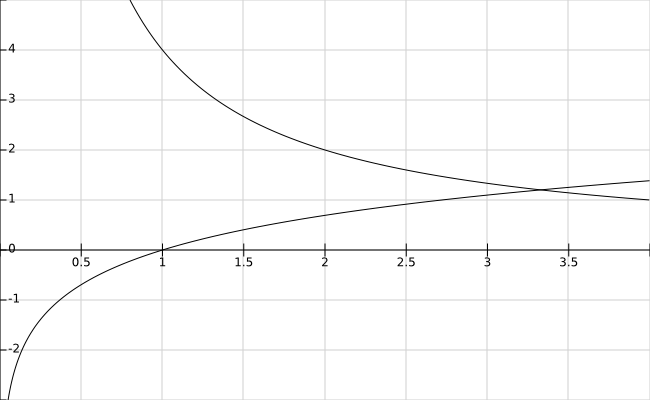
\includegraphics[scale=.666]{6.png}\\
    Area:\\
    "Big": $\frac{4}{x}$\\
    "Small": $\ln{x}$\\
    $=\int_{1}^{3}\! \frac{4}{x} - \ln{x} \, \dx$\\
    $=\ln{3} + 2$\\
    \paragraph*{9:\\}
    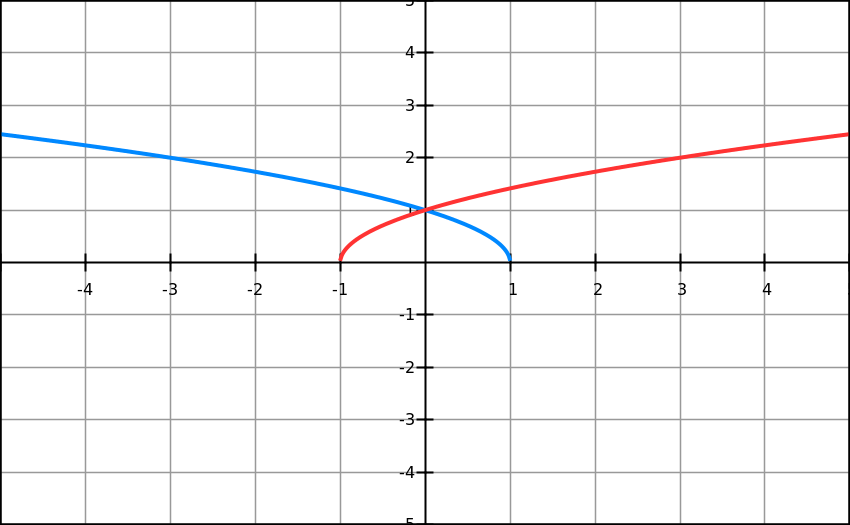
\includegraphics[scale=.666]{9.png}\\
    $f(x) = \sqrt{-x+1}$\\
    $g(x) = \sqrt{x+1}$\\
    No upper function:
    $f(x)$ larger from $(-1, 0)$, $g(x)$ larger from $(0, 1)$\\
    $\int_{-1}^{0} \! f(x) - g(x) \, \dx + \int_{0}^{1} \! g(x) - f(x) \, \dx$\\
    $\int_{-1}^{0} \! \sqrt{-x+1} - \sqrt{x+1} \, \dx + \int_{0}^{1} \! \sqrt{x+1} - \sqrt{-x+1} \, \dx$\\
    $= \frac{8\sqrt{2} - 8}{3}$\\
    \paragraph*{15:\\}
    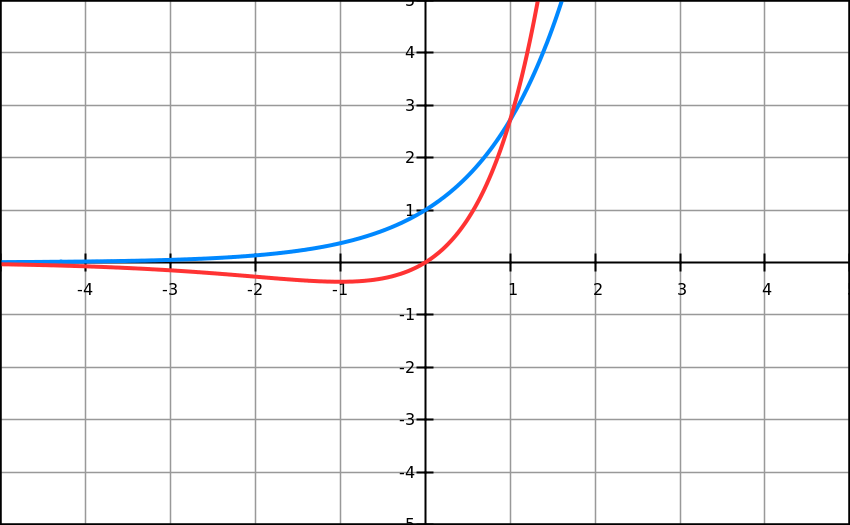
\includegraphics[scale=.666]{15.png}\\
    $\int_{0}^{1} \! \me^x - x\me^x \, \dx$\\
    $= 1$\\
    \paragraph*{21:\\}
    $[1, \frac{4}{3}]$\\
    $\int_{0}^{1/3} \! \sqrt{x-1} - x^2 \ln x \, \dx$\\
    $\approx 0.05$\\
    \paragraph*{22:\\}
    $[0, 1]$\\
    $\int_{0}^{1} \! x\cdot\cos{x} - x^{10} \, \dx$\\
    $\approx 0.3$\\
    \paragraph{23:\\}
    $f(x) = \cos{x}\\g(x) = \sin{2x}$\\
    $\int_{0}^{1/2} \! \cos{x} - \sin{2x} \, \dx + \int_{1/2}^{1} \! \sin{2x} - \cos{x} \, \dx$\\
    $\approx 0.37$
    \paragraph*{26:\\}
    \subparagraph*{a:}
    Car $A$; it has traveled a greater distance
    \subparagraph*{b:}
    Distance between car $A$ and $B$
    \subparagraph*{c:}
    Can't tell. Car $B$ is at a higher velocity, but that doesn't mean it's ahead.
    \subparagraph*{d:}
    2 minutes?
    \paragraph*{27:\\}
    $\Delta x = 2$\\
    $\frac{\Delta x}{3} \cdot [1\cdot0 + 4\cdot6.2 + 2\cdot7.2 + 4\cdot6.8 + 2\cdot5.6 + 4\cdot5.0 + 2\cdot4.8 + 4\cdot4.8 + 1\cdot0]$
    $= \frac{2}{3} \cdot 126.4$\\
    $\approx 84.27$
    \paragraph*{29:\\}
    $\approx 8868$. Equals the amount of population growth over 10 years.
    \paragraph*{30:\\}
    The shaded region is total profit

    % \paragraph*{6.1:} 2, 3, 6, 9, 15, 17, 21, 22, 23, 26, 27, 29, 30
    % \paragraph*{6.2:} 1, 2, 3, 5, 9, 14, 16, 20, 21, 25, 26, 28, 31, 33
\thispagestyle{fancy}

\end{document}

